\newcommand{\Nnoisy}{500}
\newcommand{\Nnoisefree}{500}
\newcommand{\kepler}{{\it Kepler}}

% \section{Introduction}

The light curves of spotted, rotating stars are often non-sinusoidal and
Quasi-Periodic (QP).
These stars vary in brightness due to active regions on their surfaces which
rotate in and out of view.
The non-sinusoidal quality is caused by the complicated surface spot patterns
and the quasi-periodicity is caused both by the finite lifetimes of these
active regions and the presence of differential rotation.
A strictly periodic sinusoid is therefore not a good representative
model for the light curves of FGK stars.
In an ideal world, a physical model of the stellar surface would be
conditioned on the data.
A physically realistic generative model would perfectly capture the
complexity of shapes within stellar light curves as well as the
quasi-periodic nature, allowing for extremely precise probabilistic period
recovery.
However, such physical models must have many free parameters in order to
accurately represent a stellar surface and these parameters are extremely
degenerate.
For example, as well as global stellar parameters such as inclination and
rotation period, each spot or active region should have (at minimum) a
longitude, latitude, size, temperature and lifetime.
Considering that many stars have on the order of hundreds of spots CITATION,
the number of free parameters quickly becomes unwieldy, especially if the
posterior PDFs of these parameters are explored with MCMC.
Simplified spot models, such as the one described in \citet{lanza}, where
only two spots are modelled, have produced successful results, however these
simplified models sacrifice some precision due to lack of model flexibility.
Instead of using a physical model for stellar light curves, we choose to use
an {\it effective} model.
One which captures the behaviour but is not physically motivated (although
the parameters of this model may be interpreted as physical ones).
An ideal effective model for the light curve of a spotted, rotating star is
one with a small number of non-degenerate parameters that is flexible enough
to perfectly capture non-sinusoidal, QP behaviour.
These requirements are perfectly fulfilled by a Gaussian process (GP) model.

The standard methods used for measuring rotation perids are detecting peaks in
a Lomb-Scargle (CITATION) (LS), sine-fitting periodograms
\citep[e.g.][]{reiners}, Auto-Correlation Functions (ACFs)
\citep{mcquillan2013} and wavelet transforms \citep{garcia2014}.
The efficacy of the LS periodogram and the wavelet methods are limited by the
suitability of the model choice.
In the case of the LS periodogram, the sinusoid is not an ideal model, as
described above, and the wavelet method similarly relies on a choice of mother
wavelet that should match the data over a range of transpositions.
The ACF method is much better suited to signals that are non-sinusoidal, in
fact it doesn't matter what shape the signal is---as long as it is periodic,
the ACF will contain peaks located at the period.
However, the ACF method requires data to be evenly-spaced, which is not the
case with \Kepler light curves (although in many cases it can be approximated
as uniformly sampled).
It is also an operation performed on the data, not a generative model of the
data and is therefore not probabilistic.
It is very difficult to estimate the uncertainty on a rotation period
measurement for this reason.
Many rotation periods in the literature have been inferred by measuring the
position in the first peak of an ACF, however this approach can be dangerous.
The exponential decay in correlation can shift the peak position to the left
of its true value, leading to an underestimate of the period.
In order to avoid this, a period should be inferred by modelling the entire
ACF, not just measuring the position of the first peak.

The motivation for developing a GP-based method for rotation period inference
is firstly, to measure more accurate and precise rotation periods using a
better-suited generative model than a sine-fitting periodogram for the
reasons explained above.
Secondly, to infer {\it probabilistic} periods, i.e. to estimate the
posterior PDF of the rotation period and thereby measure a realistic and
representative uncertainty.
Thirdly, to allow for an additional noise model to be included during
regression, the parameters of which could be marginalised over.
Fourthly to provide some way of determining whether a periodic model is
supported by the data over a purely stochastic one.

GPs are commonly used in the machine learning community and increasingly
in other scientific fields, for example biology and geophysics (where GP
regression is called `krigging').
They are useful in regression problems involving a stochastic process,
specifically when the probability distribution for the process is a
multi-variate Gaussian.
If the probability of obtaining a data set, generated by some process, is a
Gaussian in $N$ dimensions, where $N$ is the number of data points, that data
set can be described as and {\it with} a Gaussian process.
Gaussian process models parameterise the covariance between data points to
describe the data.
A kernel function provides the parameterisation of the covariance matrix.
For example, take the time-series in figure \ref{fig:GP_example}.
This is a \kepler\ light curve of Earth-like planet host Kepler-452, a G-type
star that rotates once every $\sim$ 15 days.
The variability visible in this time-series is typical of \kepler\ FGK stars.
It has been fit with a GP model, shown in orange.
Since GPs are flexible models, a range of kernel functions could be used to
describe the variability of Kepler-452.
For example, the simplest and most commonly used kernel function, the
'Squared Exponential' (SE) could produce an adequate fit to these data.
The SE kernel function is defined as,
\begin{equation}
k_{i,j} = A \exp \left(-\frac{(x_i - x_j)^2}{2l^2} \right).
\end{equation}
\label{eq:SE}
The SE kernel function has the advantage of being very simple---it has just
two parameters, $A$, the amplitude of covariance and $l$ the exponential
length scale of covariance decay.
If $l$ is large, two data points very far apart in $x$ will be tightly
correlated, and vice versa.
The SE kernel function may be an adequate model of the covariance in stellar
light curves, but it is not a `useful' one because it does not have a
parameter that controls a period.
In order to infer a rotation period, it is necessary to use a periodic kernel
function and to optimise the parameter that controls the period.
For this reason, we use the `Quasi-Periodic' (QP) kernel function for the
inference of stellar rotation periods.
The QP kernel function is defined as
\begin{equation}
k_{i,j} = A \exp \left(-\frac{(x_i - x_j)^2}{2l^2} -
\frac{\sin(\frac{2\pi}{P})^2}{\Gamma^2} \right).
\end{equation}
\label{eq:QP}
It is the product of the SE kernel function which describes the overall
covariance decay and an exponentiated, squared, sinusoidal kernel function,
that describes the periodic covariance structure.
$P$ can be interpreted as the rotation period of the star and $\Gamma$ is
related to the number of zero crossings per period.
$\Gamma$ may be related to the number of active regions on the stellar
surface, however investigating the connections of these hyper-parameters to
physical properties of the stars (other than rotation period) is beyond the
scope of this project.
This kernel function allows two data points that are separated in time by one
rotation period to be tightly correlated, while points separated by half a
period are weakly correlated.
This kernel function was used to produce the orange model shown in figure
~\ref{fig:GP_example}.
In order to infer a stellar rotation period from a light curve, a GP model
with a QP covariance function is fit to the data.
The likelihood of the model, conditioned on the data could then be maximised
in order to find the maximum likelihood value for $P$.
Alternatively, and as we do in this study, the posterior PDFs of the
hyper-parameters are explored using MCMC.
This latter approach comes at a cost: a GP model is expensive to compute
once, let alone however many thousands of times is necessary to fully explore
the posteriors of the parameters.
However, it fully maps out the posterior PDF of $P$, which is one of the
primary goals of this alternative approach to rotation period inference.

\begin{figure}
\begin{center}
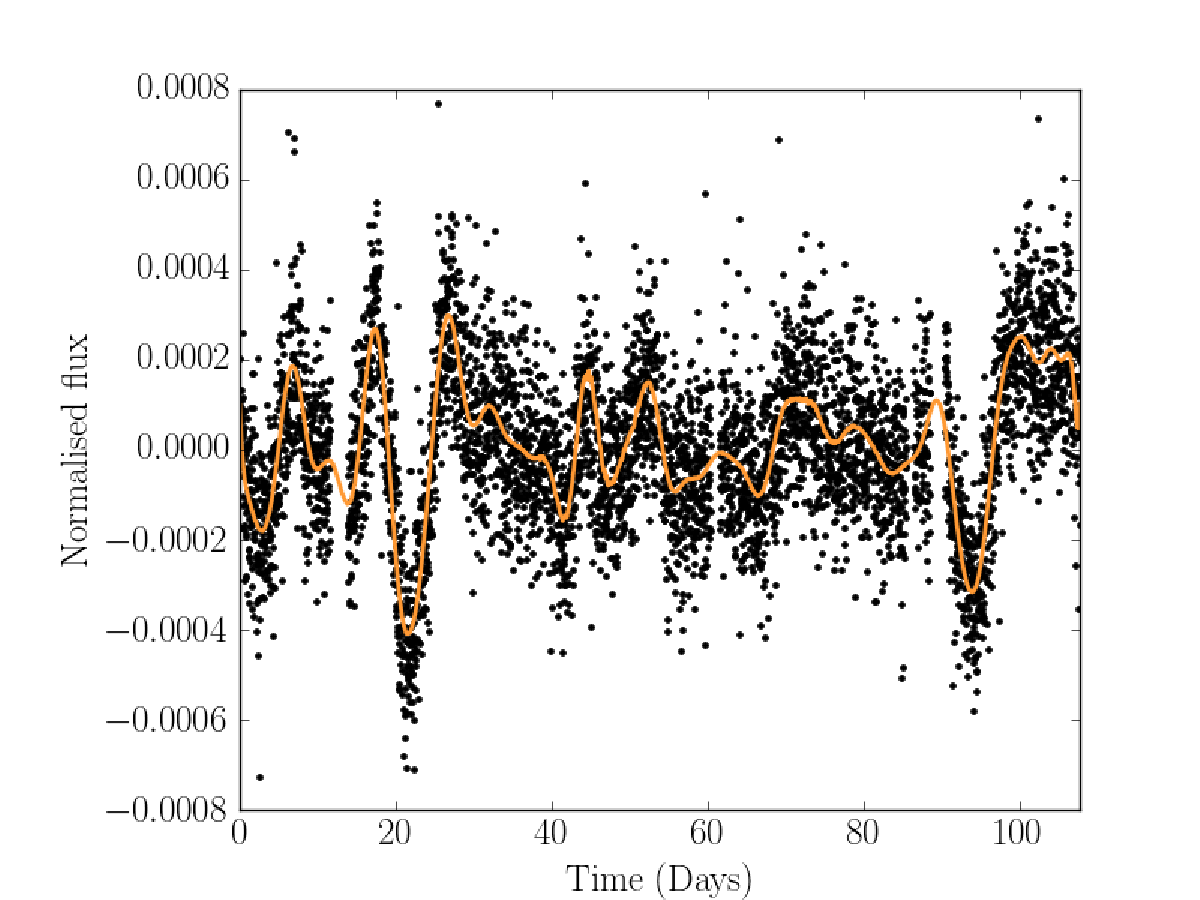
\includegraphics[width=6in, clip=true]{figures/Kepler452b.pdf}
\caption{Light curve of Kepler-452 b, a habitable-zone, Earth-sized planet
hosting G star \citep{jenkins}. The orange line shows a fit to the data using
a Gaussian process model with a QP covariance kernel function.}
\label{fig:GP_example}
\end{center}
\end{figure}

\section{Simulations}

In order to infer a rotation period from a light curve, we attempted to
measure rotation periods of three sets of light curves: simulated noise-free,
simulated noisy and real light curves.

We simulated realistic light curves using a simplified version of the code
used by \citet{aigrain15}.

We simulated \Nnoisefree noise-free light curves with rotation periods between
... and ... days.
These simulated light curves were then injected into the light curves of
quiet \Kepler stars in order to attempt to recover signals from light curves
with \Kepler-like systematics.
Ideally, we would inject simulated light curves into the pixel-level data,
then apply the same detrending techniques to the data before attempting to
measure rotation periods for these stars.
However, since this work is designed to be more of a demonstration of the
efficacy of the GP periodogram, rather than the development of a \Kepler data
specific method, this is beyond the scope of our demonstrations.

\begin{figure}
\begin{center}
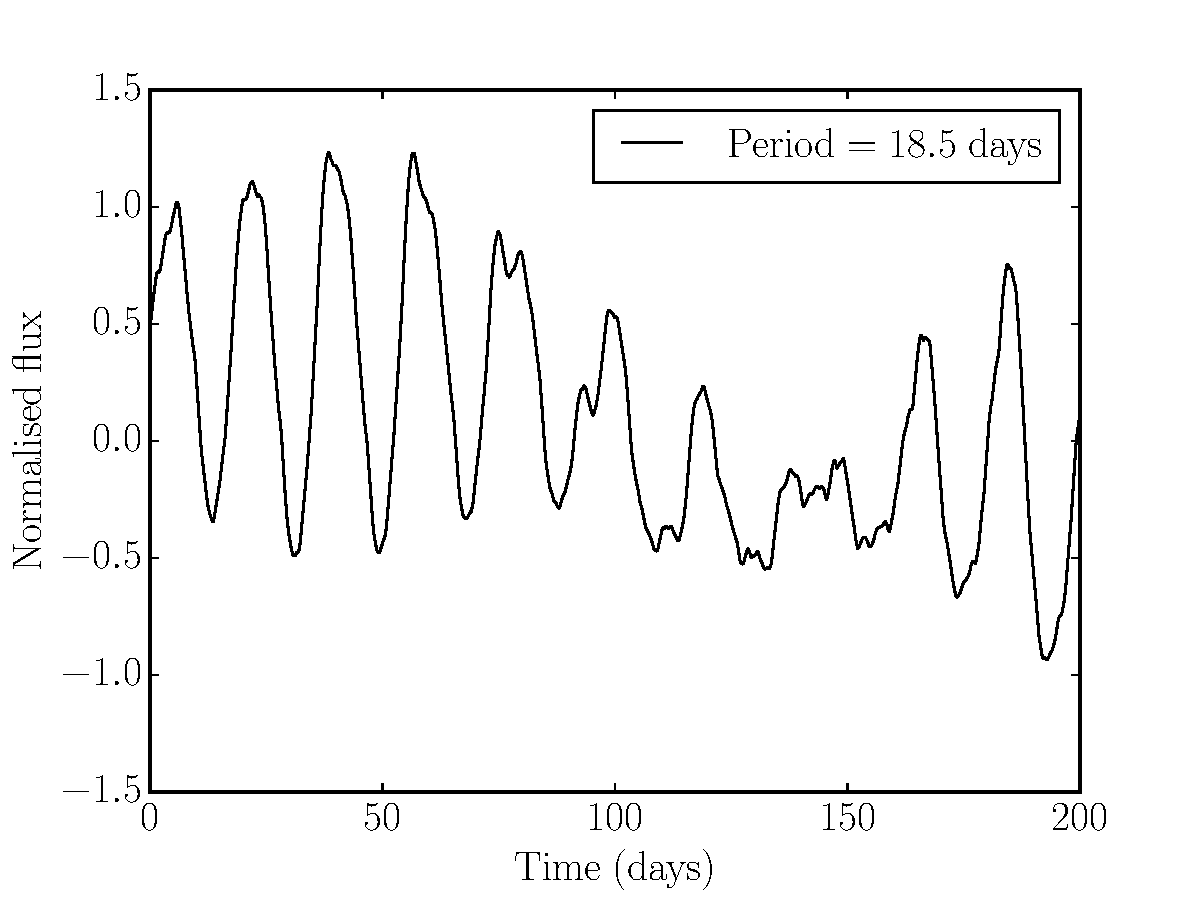
\includegraphics[width=6in, clip=true]{figures/noise-free_lc.pdf}
\caption{An example simulated light curve. This `star' has a rotation period
of ... days.}
\label{fig:noise-free_lc}
\end{center}
\end{figure}

Figure \ref{fig:noise-free_lc} shows an example of a simulated, noise-free
light curve with a period of ... days.

\section{Rotation period recovery}

In order to estimate an initial guess for the rotation period we calculated an
ACF for each light curve using the method of \citet{mcquillan13}.
A rotation period is estimated from the ACF as the lag-time of the first peak,
unless the second peak is larger in which case that lag-time is interpreted as
the true period.
The second peak in an ACF can be larger than the first if there are two
active regions at opposite longitudes on the surface of the star.
This would produce a light curve with two dips per rotation period.
Using the ACF period as an initial guess, we then subsample the light curves
and split them into \kepler quarters in order to reduce computation time.
The subsampling reduces computation time simply by contracting the data
set---the HODLR solver scales as $N \log ^2 (N)$.
Splitting the data set into quarters, rather than modelling the entire time
series contiguously also speeds up the computation time as inverting several
small matrices is faster than inverting one large one.
The \kepler quarter divisions are natural places to split the time series
because the spacecraft rotates by ninety degrees every quarter (three months),
placing each star on a new CCD module.
Pixel response functions and background flux differs from pixel-to-pixel and
module-to-module, so noise properties of \kepler light curves change every
quarter.
Additionally, changes in the spacecraft's orientation and position during
quarterly re-pointings temporarily affect the temperature of the CCD,
producing systematic features in the light curves at the start of some
quarters.

We model each quarter separately, however the parameters of the GP kernel
function are global, {\it i.e.} we do not use a separate period parameter for
each quarter---there is just one period parameter for an entire light curve.
It would be possible to model the time series with a mixture of some global
parameters and some quarter-specific parameters, for example one might expect
that the amplitude of covariance, $A$ or white noise level, $\sigma$ to vary
on a quarterly basis.
However, since there are seventeen quarters this would lead to thirty-seven
parameters, and in the interest of minimising computation time (adding
parameters leads to longer MCMC burn in and convergence time), we choose to
use global parameters only.

BENCHMARK

Example light curve figure.
Example ACF.
Example GP fit.
Corner plot.
